% Created 2014-03-01 Sat 16:08
\documentclass[11pt]{report}
\usepackage[utf8]{inputenc}
\usepackage[T1]{fontenc}
\usepackage{fixltx2e}
\usepackage{graphicx}
\usepackage{longtable}
\usepackage{float}
\usepackage{wrapfig}
\usepackage{rotating}
\usepackage[normalem]{ulem}
\usepackage{amsmath}
\usepackage{textcomp}
\usepackage{marvosym}
\usepackage{wasysym}
\usepackage{amssymb}
\usepackage{hyperref}
\tolerance=1000
\usepackage{minted}
\usepackage[bibstyle=numeric,citestyle=authoryear,backend=biber]{biblatex}
\addbibresource{bibliography.bib}
\usepackage[]{hyperref}
\hypersetup{hidelinks}
\usepackage[]{nomencl}
\author{Volker Strobel}
\date{\today}
\title{Knowledge Engineering Tools for Planning in PDDL - Syntax Highlighting, Task Generation and Plan Visualization and Execution - an extensible framework}
\hypersetup{
  pdfkeywords={},
  pdfsubject={},
  pdfcreator={Emacs 24.3.1 (Org mode 8.2.5h)}}
\begin{document}

\maketitle
\tableofcontents

\begin{abstract}
Automated planning and scheduling blazes a trail for artificial
intelligent behavior. PDDL, a planning language widely used for AI
task specifications requires extensive knowledge engineering effort.
After giving an overview of PDDL syntax and planning basics, a plug-in
(including syntax highlighting) for the code editor Sublime Text and
related editors will be given. A type diagram generator will be
presented that supports modeling of the environment. The usability of
these tools will be evaluated by subjects without prior knowledge in
PDDL. By the use of these tool, the average modeling time of a shorter
task specification could be improved by \ldots{} percent and the error rate
could be reduced from \ldots{} to \ldots{} . Furthermore, this thesis will
present approaches for the automatic generation of task specifications
and provide a basic interface between the functional programming
language Clojure and PDDL. The proposed tools can assist knowledge
engineers in the design process.

\url{https://www.ece.cmu.edu/~koopman/essays/abstract.html}
\end{abstract}
\chapter{Introduction}
\label{sec-1}
\begin{center}
\fbox{
\begin{minipage}[c]{.6\textwidth}
TODO:

\rule[.8em]{\textwidth}{2pt}

\begin{itemize}
\item Scope of the article (What did I miss out, what is included?)
\item Name Tools and provide found possibilities and limitations
\item Motivation: Why is this article interesting?
\item Structure of the article
\item Review of relevant literature? Note: I can review the relevant
literature and related work in the related chapter, if this is
convenient
\item Planning Architecture - 3 Tier Architecture
\item ICAPS
\item Handicapped people -> Planning Interaction
\item Why is something interesting? -> reasons! (and not because it does
not exist yet)
\end{itemize}
\end{minipage}
}
\end{center}

Planning is one the the classic Artificial Intelligence (AI) tasks.
Knowledge engineering (KE), that means representing world information
in a computer system, is the crucial step for utilizing AI planning
systems to solve problems. By definition (TODO: \ldots{}), it requires an
human expert who knows the underlying syntax and models the
information manually. This process is naturally error-prone and
time-consuming. While planning systems are improving steadily (\ldots{}),
the main work for useful systems lies on the representing language.
The Planning Domain Definition Language (PDDL)
\parencite{mcdermott1998pddl} allows for a standardized way of
specifying planning tasks. While on the one hand, recent PDDL
extensions \parencite{fox2003pddl2,kovacs2011bnf} extended the
expressiveness of PDDL and tackle a route for real-world applications,
they also demand a higher level of knowledge and attention of the
knowledge engineer. Particularly with the start in 2005 of the
International Competition on Knowledge Engineering for Planning and
Scheduling (ICKEPS), new tools for the shift from at the modeling
process from a text based 'programming paradigm' to a user-friendly
graphical design tool exist, however, they also arouse drawbacks:
limited functionality, expenditure of time, editing difficulty, to
name a few. As in other computer languages, so far, there is no real
way around diving into the 'code paradigm'. Despite recent advances in
the area, the performance of planning \& scheduling systems is still
dependent to a large extent on how problems and domains are
formulated, resulting in the need for careful system fine-tuning
(copied 1:1). This thesis will, after introducing the basic terms and
definitions of PDDL, focus on the software support for knowledge
engineers. A package for the text and source code editor Sublime Text
(ST) will be introduced, that provides syntax highlighting and PDDL
templates. And the functionality is transferred to a on-line editor
with instant access. Together with this package, a basic interface
between the functional programming language Clojure and PDDL is
developed. In this process, a UML 'type diagram' generator, derived
from UML class diagrams for Object Oriented Programming, is presented
that supports the knowledge engineer in keeping in keeping track
during the design process and gain a fast overview of existing domains
and problems.

The main focus of this thesis is about real world applications and the
development of handy tools that support (and partially automatize) the
planning process. 
\chapter{Related Work}
\label{sec-2}
\section{PDDL Studio}
\label{sec-2-1}
PDDL Studio \parencite{plch2012inspect} is an Integrated Development Environment (IDE) for
creating PDDL tasks. It was designed from scratch without, in contrast
to the work presented in this thesis, that is build on top of Sublime
Text. PDDL Studio is a pure PDDL text editor 

\section{PDDL Mode for Emacs}
\label{sec-2-2}
Announced 2005 in a mailing list entry, PDDL mode for Emacs supports
PDDL 2.2. 
\section{itSIMPLE}
\label{sec-2-3}
The itSIMPLE project is a tool that supports the knowledge engineer in
designing a PDDL domain by the use of UML diagrams. This approach is
reversed to the approach mentioned in this paper: while itSIMPLE
generates PDDL from UML, this paper generated UML from PDDL. 
\section{GIPO}
\label{sec-2-4}
\section{Pygments}
\label{sec-2-5}
\section{ModPlan}
\label{sec-2-6}
Also see VEGA plan visulazation on the MODplan page
\begin{itemize}
\item Very interesting: \url{http://www.tzi.de/~edelkamp/modplan/}
\end{itemize}

\section{VISPLAN}
\label{sec-2-7}
\chapter{Planning Basics and PDDL}
\label{sec-3}
\begin{center}
\fbox{
\begin{minipage}[c]{.6\textwidth}


\rule[.8em]{\textwidth}{2pt}

\begin{itemize}
\item Brief summary at start
\item Start with a paragraph that describes the context
\item Very interesing for basics of PDDL:
\item \url{http://www.ida.liu.se/~TDDC17/info/labs/planning/writing.html}
\item Konstruktionsanleitung
\item Propositionale Logic -> Articifial Intelligence a Modern Approach
\item To insert somewhere:
\begin{itemize}
\item It should be mentioned, that almost no planner supports every part
of PDDL. And, additionally, the quality of error messages is very
diversified. While some simple state: error occured, other list the
problem and the line.
\end{itemize}
\end{itemize}
\end{minipage}
}
\end{center}


Introduction to planing:
\url{http://books.google.de/books?id=eCj3cKC_3ikC&printsec=frontcover&dq=automated+planning&hl=en&sa=X&ei=3wgNU5fQIcHx4gSTsoDABA&redir_esc=y#v=onepage&q=automated%20planning&f=false}

AI planning describes \ldots{}

A planner and use the generated solution file (\emph{plan}).

PDDL was first described in PDDL-the planning domain definition
language (1998) and has been in constant development since then.
This thesis makes use of \textcite{pddl3.1} if not otherwise stated. 

PDDL planning task specifications are composed of two separate text files:

\begin{itemize}
\item Domain file: description of general types, predicates, functions
and actions -> uninstanciated problem independent
\item Problem file: description of a concrete problem environment -> instance specific
\end{itemize}

This separation allows for an intuitive process of task modeling:
While general instances are described in the domain file, specific
instances of problems are created in the problem files.

\begin{figure}[htb]
\centering
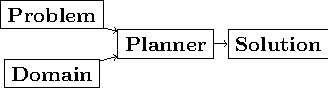
\includegraphics[width=.9\linewidth]{../img/pddl-workflow.pdf}
\caption{\label{fig:workflow}PDDL Planning workflow}
\end{figure}

These two files shell be investigated further in the following
sections.


\section{Domain File}
\label{sec-3-1}

The domain file contains the frame for planning tasks and determines,
which types, predicates and actions are possible

Domain files have a strict format: All keyword arguments must appear
in the order specified in the manual (an argument may be omitted) and
just one PDDL definition (of a domain, problem, etc.) may appear per
file. \cite[6]{fox2003pddl2}.

\begin{center}
\fbox{
\begin{minipage}[c]{.6\textwidth}


\rule[.8em]{\textwidth}{2pt}

Include simple domain -> \LaTeX{}
Include simple problem -> \LaTeX{}
Include simple plan -> not yet in \LaTeX{}
\end{minipage}
}
\end{center}

\subsection{Define}
\label{sec-3-1-1}
Every domain file starts with (define (domain <domainName>) \ldots{}) where,
<domainName> can be any string.
\subsection{Requirements}
\label{sec-3-1-2}
The requirements part is not a mandatory part of a PDDL domain file.
However, PDDL supports different "levels of expressivity", that means
subsets of PDDL features \textcite[1]{mcdermott1998pddl}. As most
planners only support a subset of PDDL the requirements part is useful
for determining if a planner is able to act on a given problem. They
are declared by the \verb~(:requirements ...)~ part. Some often used
requirements include \verb~:strips~ 
For a list of current requirement flags and their meaning, see \ldots{}

\subsection{Types}
\label{sec-3-1-3}

If order to be able to use types in a domain file, the
requirement :typing should be declared (TODO: is :adl enough?).

In order to assign categories to objects, PDDL allows for
type definitions. Like that, parameters in actions can be typed, as
well as arguments in predicates, functions [extra source!]. Later, in
the problem file, objects will be assigned to types, like objects to
classes in Object Orientated Programming (OOP). Adding to the
(:requirement \ldots{}) part of the file guarantees, that typing can be
correctly used. Strips (no types) vs ADL (types).

\subsection{Functions}
\label{sec-3-1-4}
Functions are not supported by many planners (source!) and, before
PDDL 3.1 they could only be modeled as 

It is notable that before PDDL 3.0 the keyword functors was used instead
\subsection{Actions}
\label{sec-3-1-5}
PDDL 3.1 supports two types of actions: durative-action and the
'regular' action.
\section{Problem File}
\label{sec-3-2}

Problems are designed with respect to a domain. Domains usually have
multiple problems p01.pddl, p02.pddl, \ldots{} Problems declare the initial
world state and the goal state to be reached. They instantiate types,
in they way that they create objects 
\section{Planning}
\label{sec-3-3}

A planning solution is a sequence of actions that lead from the
initial state to the goal state. PDDL itself does not declare any
uniform plan layout.

The input to the planning software is a domain and a belonging
problem, the output is usually a totally or partially ordered plan.
are software tools that Due to the yearly ICAPS, there is a broad
range of available planners. This thesis uses the planner SGPLAN\(_{\text{6}}\)
\textcite{hsu2008sgplan}, a 'extensive' (in the sense of its
supporting features) planner for both temporal and non-temporal
planning problems.

An overview of different planners is given at
\url{http://ipc.informatik.uni-freiburg.de/Planners}.
\chapter{Software Engineering Tools for AI Planning}
\label{sec-4}
\begin{center}
\fbox{
\begin{minipage}[c]{.6\textwidth}


\rule[.8em]{\textwidth}{2pt}

\begin{itemize}
\item PDDL type hierarchy and object instantiation to UML / TikZ, store
predicates (and action?) in same box as type
\item Research Knowledge Engineering in Planning
\item Human Computer Interaction
\begin{itemize}
\item \url{http://hci.waznelle.com/checklist.php}
\end{itemize}
\item Write Tiago (itSimple) regarding PDDL -> UML (and knowledge
engineering in general
\item ICKEPS (International Competition on Knowledge Engineering for
Planning and Scheduling)
\item Orient on "How to Design Classes"
\end{itemize}
\end{minipage}
}
\end{center}

\section{Statement of Problem}
\label{sec-4-1}
Writing and maintaining PDDL files can be time-consuming and
cumbersome \textcite{li2012translating}. So, the following development
tools shell support and facilitate the PDDL task design process and
reduce potential errors.

Below, methods are presented for

\begin{description}
\item[{Syntax Highlighting and Code Snippets}] Environment for Editing
PDDL files
\item[{Class Diagram Generator}] The automation of the PDDL task design process. File
input and output and dynamic generation (design level)
\item[{Human Planner Interaction}] An interactive PDDL environment: speech synthesis and
recognition.
\item[{Domain Generator}] Mathematical limitations (design level)
\end{description}
\section{Syntax Highlighting and Code Snippets}
\label{sec-4-2}
\label{sec:syntax}


Writing extensive domain and problem files is a cumbersome task:
longer files can get quickly confusing. Therefore, it is convenient to
have a tool that supports editing these files. Syntax highlighting
describes the feature of text editors of displaying code in different
colors and fonts according to the category of terms (source: Wiki). A
syntax highlighting plug-in for the text and source code editors
\textcite{sublimetext2} and \textcite{sublimetext3} is proposed and
transferred to the on-line text editor Ace are used to implement this
feature, as ST Syntax Highlighting files can easily be converted to
Ace Files. 

For Mac user, TextMate (TM) is very similar to ST and the syntax
highlighting file can be used there, too. Besides, the general
principles (e.g. regular expressions) outlined here, apply to most of
other editors as well. So, a Pygments extension was written, that
allows for syntax highlighting in \LaTeX documents.


\subsection{Implementation}
\label{sec-4-2-1}
ST syntax definitions are written in property lists in the XML format.

The syntax definition is implemented by the use of the ST plug-in
\textcite{aaapackagedev}. So, the definitions can be written in YAML
in converted to Plist XML later on.
AAAPackageDEV\textcite{aaapackagedev} is a ST plugin, that helps to
create, amongst others, ST packages, syntax definitions and 'snippets'
(re-usable code).

By means of Oniguruma regular expressions \parencite{kosako}, scopes
are defined, that determine the meaning of the PDDL code block. The
scope naming conventions mentioned in the \citetitle{textmate} are
applied here. By the means of the name, the colors are assigned.
Different ST themes display different colors (not all themes support
all naming conventions).

The syntax highlighting is intended for PDDL 3.1, but is downward
compatible, as previous versions are subsets of later versions.
\begin{center}
\fbox{
\begin{minipage}[c]{.6\textwidth}
Are later versions really subsets?

\rule[.8em]{\textwidth}{2pt}

nil\end{minipage}
}
\end{center}

The pattern matching heuristic that is implemented by the use of
regular expressions is used for assigning scopes to the parts of the
file. This heuristic is quite sophisticated, as it recognizes
sub-parts of PDDL files and chooses the color accordingly. 

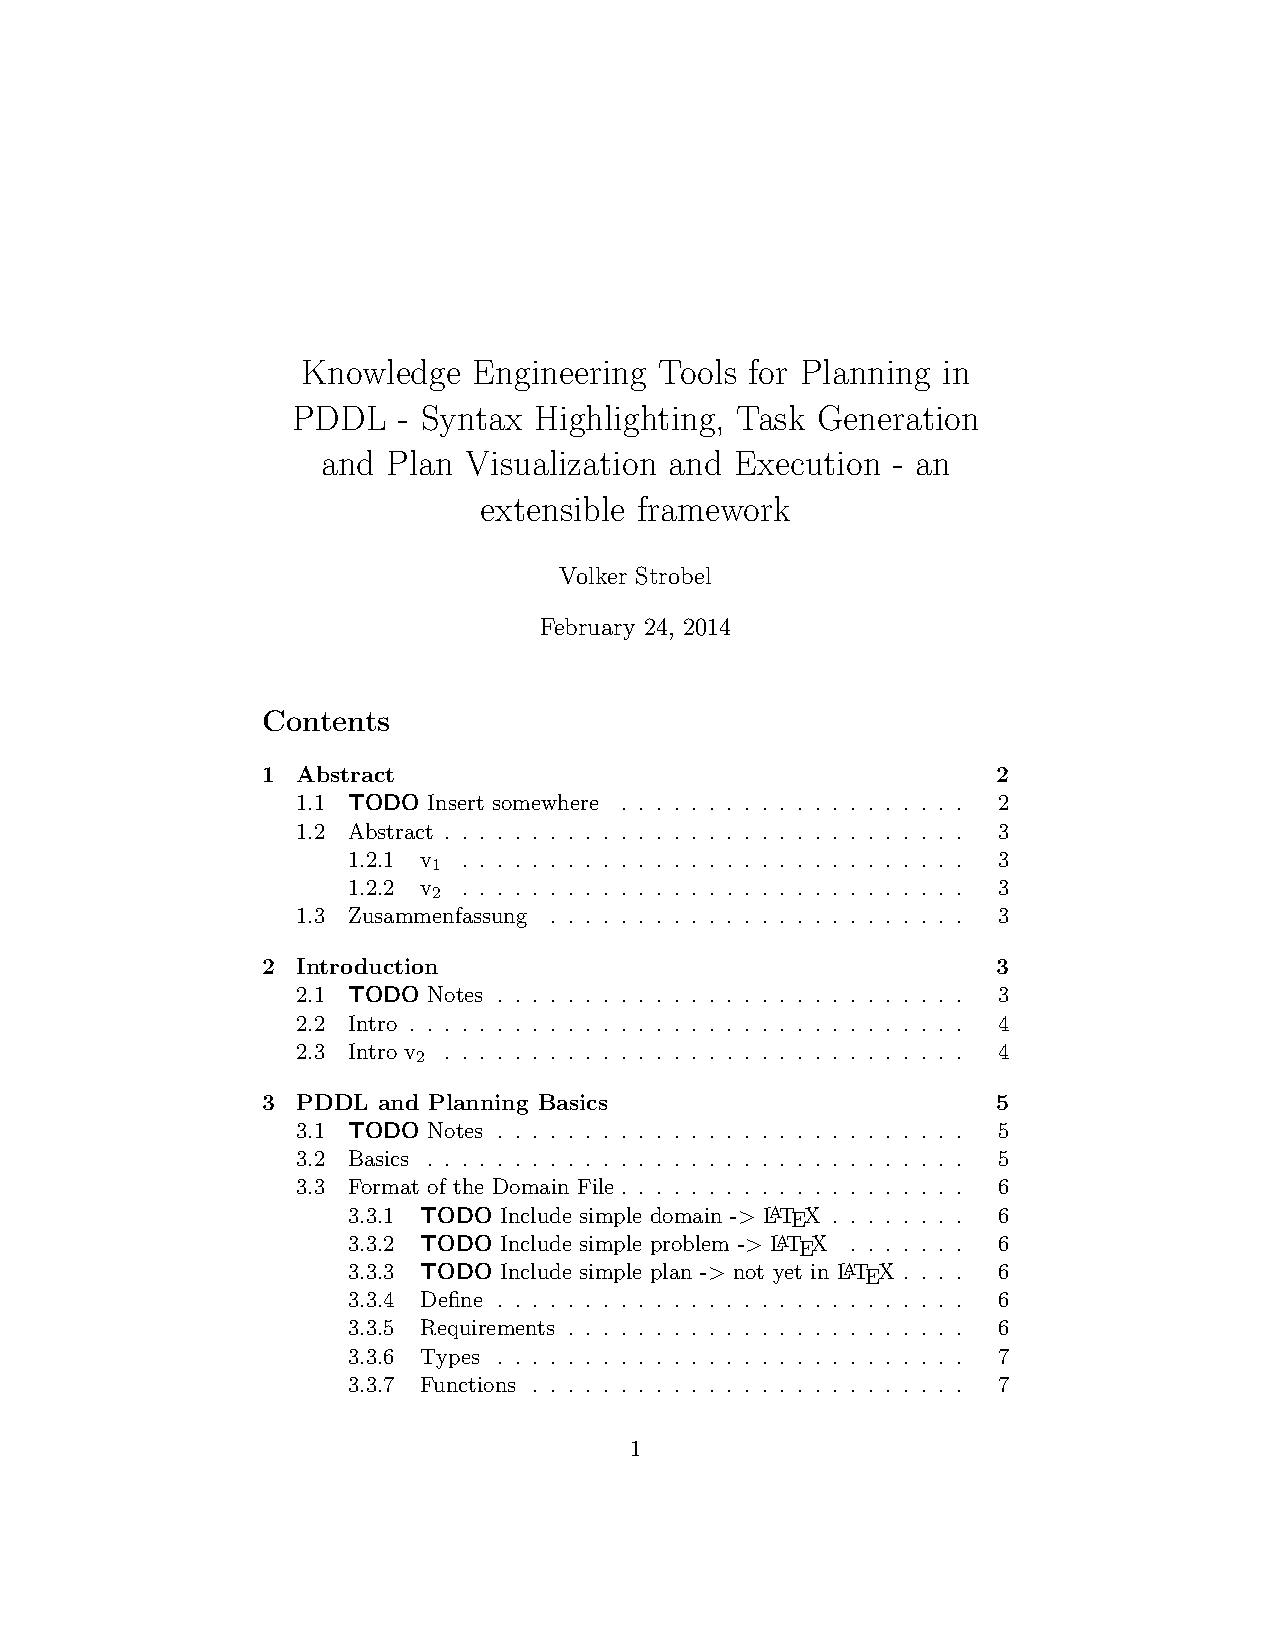
\includegraphics[width=.9\linewidth]{/home/pold/Pictures/ba.png}

\subsection{Usage and Customization}
\label{sec-4-2-2}
To enable syntax highlighting and code snippets in ST, the files of
the repository have to be placed in the ST packages folder
(\url{http://www.sublimetext.com/docs/3/packages.html}). The first part of the
PDDL.YAML-tmlanguage describes the parts of the PDDL task that should
be highlighted. By removing (or commenting) include statements, the
syntax highlighter is adjustable the user's need.

By using ST as editor, language independent ST features are supported,
like auto completion, code folding and column selection, described in
the Sublime Text 2 Documentation.



The PDDL.YAML-tmlanguage file is split in two parts:

By default, all scopes are included.

\subsection{Evaluation}
\label{sec-4-2-3}

\section{Clojure Interface}
\label{sec-4-3}

PDDL, as planning language modeling capabilities are limited, a
interface with a programming is handy a can reduce dramatically the
modeling time. In IPC, task generators are used write extensive domain
and problem files. 

As PDDL's syntax is inspired by LISP \parencite[64]{fox2003pddl2},
using a LISP dialect for the interface seems reasonable. This thesis
uses Clojure \parencite{hickey2008clojure}, a modern LISP
dialect that runs on the Java Virtual Machine.

In this section, I will not only show a method for generating PDDL
constructs, but also for reading in PDDL files are handling the input.

\subsection{Basics}
\label{sec-4-3-1}
Through the higher-order filter method in Clojure, parts of PDDL files
can be easily extracted. Like that, one can extract parts of the file
and handle the constructs in a Clojure intern way.

As an example, the type handling will be represented here, but the
basic approach is similar for all PDDL constructs.

The here developed tools should be platform independent with a
development focus in UNIX/Linux systems, as most planners (source!)
run on Linux.
\subsection{Functions}
\label{sec-4-3-2}
As functions have a return value, the modeling possibilities
dramatically increase.

\subsection{Numerical Expressiveness}
\label{sec-4-3-3}
One might assume that the distance could be modeled as follows:

\begin{verbatim}
(durative action ...
...
  :duration (= ?duration (sqrt (coord-x )))
...
\end{verbatim}

However, PDDL does only support basic arithmetic operations (+, -, /, *).

An Euclidean distance function that uses the square root would be
convenient for distance modeling and measurement. However, PDDL 3.1
supports only four arithmetic operators (+, -, /, *). These
operators can be used in preconditions, effects
(normal/continuous/conditional) and durations.
\textcite{parkinson2012increasing} describe a workaround for this
drawback. By declaring an action `calculate-sqrt', they bypass the
lack of this function and rather write their own action that makes use
of the Babylonian root method.

\begin{enumerate}
\item Alternative \#1: Only sqrt exists
\label{sec-4-3-3-1}
Assuming that a function sqrt would actually exist, the duration could be modeled as follows:

\begin{verbatim}
:duration (= ?duration 
             (sqrt
              (+
               (*
                (- (pos-x (current-pos))
                   (pos-x ?goal))
                (- (pos-x (current-pos))
                   (pos-x ?goal)))
               (*
                (- (pos-y (current-pos))
                   (pos-y ?goal))
                (- (pos-y (current-pos))
                   (pos-y ?goal))))))
\end{verbatim}
\item Alternative \#2: sqrt and expt exist
\label{sec-4-3-3-2}
Assuming that a function sqrt would actually exist, the duration could be modeled as follows:
\begin{verbatim}
:duration (= ?duration 
             (sqrt
              (+
               (expt
                (- 
                 (pos-x (current-pos))
                 (pos-x ?goal)))
               (expt
                (- 
                 (pos-y (current-pos))
                 (pos-y ?goal))))))
\end{verbatim}

\item Alternative \#3: Calculate distance and hard code it, e.g. (distance table kitchen) = 5.9
\label{sec-4-3-3-3}

\begin{itemize}
\item Distance Matrix
\item \url{http://stackoverflow.com/questions/20654918/python-how-to-speed-up-calculation-of-distances-between-cities}
\item Scipy.spatial.distance (-> Clojure?)
\item Mention that the Taxicab geometry allows different ways that have an equal length
\end{itemize}

Another alternative is to make use of an external helper and, instead
of calculating every entry of the distance matrix. the distance only
if needed, incorporate every possible combination of two locations.
This approach has certainly a major drawback: With an increasing
amount of locations, the number of combinations increases
exponentially. That means, if there are 100 locations, there will be
\begin{center}
\fbox{
\begin{minipage}[c]{.6\textwidth}
TODO: Calculate possibilities

\rule[.8em]{\textwidth}{2pt}

nil\end{minipage}
}
\end{center}
\ldots{} . The native approach would be to iterate over the cities twice
and calculate only the half of the matrix (as it is symmetric, that
mean distance from A to B is the same as the distance from B to A).

\item Alternative \#4: Use the Manhattan distance
\label{sec-4-3-3-4}

Allowing the agent to move only vertically and horizontally would be
that one can use the so called Taxicab geometry (or Manhattan length)
as distance measurement.  In the Kitchen domain, this could be modeled
as follows:

\begin{verbatim}
% => Metric: reduce duration

% dKitchenware.pddl 
\begin{figure}[t]
\inputminted[mathescape, linenos, numbersep=5pt, frame=lines, framesep=2mm]
            {csharp}
            {Code/dKitchenware.pddl}
\caption{The basic kitchenware domain}
\end{figure}
\section
\end{verbatim}

\begin{center}
\fbox{
\begin{minipage}[c]{.6\textwidth}
TODO:

\rule[.8em]{\textwidth}{2pt}

TODO Human Planner Interaction
\end{minipage}
}
\end{center}
\end{enumerate}
\section{Type Diagram Generator}
\label{sec-4-4}
\begin{center}
\fbox{
\begin{minipage}[c]{.6\textwidth}


\rule[.8em]{\textwidth}{2pt}

Add actions to the Type Diagram?
\end{minipage}
}
\end{center}

Graphical notations, have some advantages compared to textual
notations, as they simplify the communication between developers and
help to quickly grasp the connection of related system units. 

But for all that one disadvantage has to be accepted: 

The UML was invented in order to standardize modeling in software
engineering (SE). The UML consists of several part notations, the here
presented tool uses the 'class diagram' notation, as PDDL types and
classes in OOP have strong resemblance (see Tiago 2006, p 535). 

Types play a major role in the PDDL design process: they are involved,
besides their definition, in the constants, predicates and actions
part. So, a fine grasp of their hierarchy, as well as their involved
predicates becomes handy and assists the KE in the planning process.
Types strongly resemble classes in object oriented programming
As mentioned in chapter (\ldots{}), the type definitions follow a specific
syntax. For example \verb~truck car - vehicle~ would indicate, that both
\verb~truck~ and \verb~car~ are subtypes of the super-type vehicle. 

Subtypes and corresponding super-types can be extracted using regular
expressions. \#"(\ldots{}.)" matches every kind of that form and a
Clojure-friendly representation in form of a hash-map can be created.

PDDL side ----------------------------------------------- Clojure side

'(:types \ldots{} \ldots{} --- \ldots{})                      \{\ldots{} [\ldots{} \ldots{} \ldots{}], \ldots{}\}

\begin{figure}[htb]
\centering
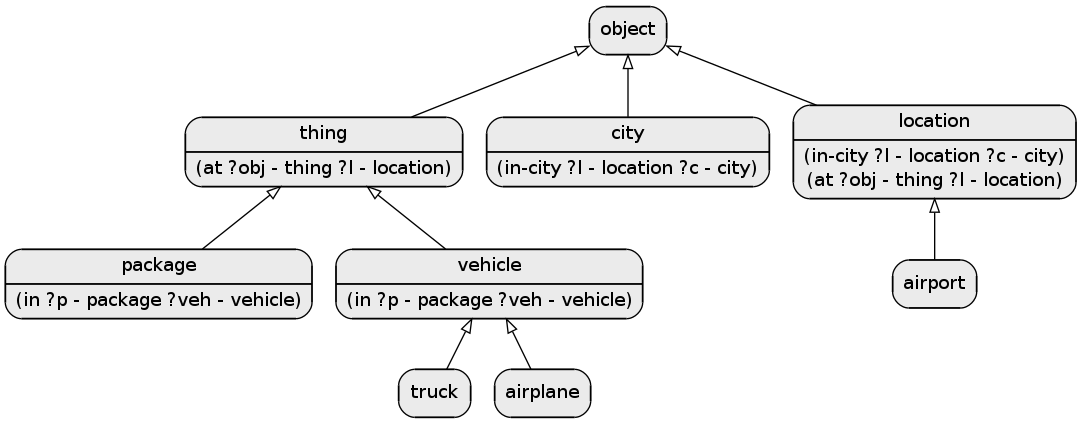
\includegraphics[width=.9\linewidth]{/home/pold/Documents/BA/org-ba/diagram.png}
\caption{Part of a PDDL domain and the corresponding, generated UML diagram}
\end{figure}

\chapter{Analysis}
\label{sec-5}
\section{Participants}
\label{sec-5-1}
Ten non-paid students (six female) took part in the experiment. All
had knowledge about LISP syntax, but neither one had faced PDDL prior
to this study. 
\section{Material}
\label{sec-5-2}
The usability of the Syntax Highlighter (see \ref{sec:syntax}) and the Type
Diagram Generator (see \texttt{Type Diagram Generator}) were
tested.
\section{Design}
\label{sec-5-3}

The participants had to 

\section{Procedure}
\label{sec-5-4}
\chapter{Conclusion and Outlook}
\label{sec-6}
The tools presented in this thesis have been designed to support
knowledge engineers in planning tasks. They can support engineers in
the early planning design process, as well as in the maintenance of
existing domains and problems. The communication between engineers can
be facilitated and 


\section{Outlook}
\label{sec-6-1}
Besides ICKEPS, as mentioned in the introduction, also the yearly
workshop Knowledge Engineering for Planning and Scheduling (KEPS) will
promote the research in planning and scheduling technology. Potentially, the main effort of
for implementing models in planning will be shifted from the manual KE
to the automated knowledge acquisition (KA). Perception systems,
Nevertheless, a engineer who double-checks the generated tasks will be
irreplaceable.  
\printbibliography

\chapter{Appendix}
\label{sec-7}
\(\alpha\)
% Emacs 24.3.1 (Org mode 8.2.5h)
\end{document}